%==============================================================================00
% Options for packages loaded elsewhere
\PassOptionsToPackage{unicode}{hyperref}
\PassOptionsToPackage{hyphens}{url}
%==============================================================================01
\documentclass[11pt, oneside, openany]{scrbook}
\setkomafont{disposition}{\bfseries}
\usepackage{mathptmx}
\usepackage{lipsum}
%==============================================================================03
% Make chapter pages have numbering at top right
\usepackage{fancyhdr}
\pagestyle{fancy}
\lhead{}
\chead{}
\rhead{\thepage}
\lfoot{}
\cfoot{}
\rfoot{}
\renewcommand{\headrulewidth}{0pt}
\makeatletter
\renewcommand\chapter{\if@openright\cleardoublepage\else\clearpage\fi
                    \thispagestyle{fancy}%
                    \global\@topnum\z@
                    \@afterindentfalse
                    \secdef\@chapter\@schapter}
\makeatother
%==============================================================================03
\usepackage{lmodern}
\usepackage{setspace}
%==============================================================================04
\usepackage{amssymb,amsmath}
%==============================================================================05
\usepackage{ifxetex,ifluatex}
\ifnum 0\ifxetex 1\fi\ifluatex 1\fi=0 % if pdftex
  \usepackage[T1]{fontenc}
  \usepackage[utf8]{inputenc}
  \usepackage{textcomp} % provide euro and other symbols
\else % if luatex or xetex
  \usepackage{unicode-math}
  \defaultfontfeatures{Scale=MatchLowercase}
  \defaultfontfeatures[\rmfamily]{Ligatures=TeX,Scale=1}
\fi
%==============================================================================06
% Use upquote if available, for straight quotes in verbatim environments
\IfFileExists{upquote.sty}{\usepackage{upquote}}{}
\IfFileExists{microtype.sty}{% use microtype if available
  \usepackage[]{microtype}
  \UseMicrotypeSet[protrusion]{basicmath} % disable protrusion for tt fonts
}{}
\makeatletter
\@ifundefined{KOMAClassName}{% if non-KOMA class
  \IfFileExists{parskip.sty}{%
    \usepackage{parskip}
  }{% else
    \setlength{\parindent}{0pt}
    \setlength{\parskip}{6pt plus 2pt minus 1pt}}
}{% if KOMA class
  \KOMAoptions{parskip=half}}
\makeatother
%==============================================================================07
\usepackage[table]{xcolor}
%==============================================================================08
\IfFileExists{xurl.sty}{\usepackage{xurl}}{} % add URL line breaks if available
\IfFileExists{bookmark.sty}{\usepackage{bookmark}}{\usepackage{hyperref}}
\hypersetup{
  pdftitle={Contributions to Modern Bayesian Multilevel Modeling},
  pdfauthor={Alexander Knudson},
  hidelinks,
  pdfcreator={LaTeX via pandoc}}
\urlstyle{same} % disable monospaced font for URLs
%==============================================================================09
\usepackage[top=1in, left=1.5in, bottom=1.25in, right=1.5in]{geometry}
%==============================================================================10
\usepackage{color}
\usepackage{fancyvrb}
\newcommand{\VerbBar}{|}
\newcommand{\VERB}{\Verb[commandchars=\\\{\}]}
\DefineVerbatimEnvironment{Highlighting}{Verbatim}{commandchars=\\\{\}}
% Add ',fontsize=\small' for more characters per line
\usepackage{framed}
\definecolor{shadecolor}{RGB}{248,248,248}
\newenvironment{Shaded}{\begin{snugshade}}{\end{snugshade}}
\newcommand{\AlertTok}[1]{\textcolor[rgb]{0.94,0.16,0.16}{#1}}
\newcommand{\AnnotationTok}[1]{\textcolor[rgb]{0.56,0.35,0.01}{\textbf{\textit{#1}}}}
\newcommand{\AttributeTok}[1]{\textcolor[rgb]{0.77,0.63,0.00}{#1}}
\newcommand{\BaseNTok}[1]{\textcolor[rgb]{0.00,0.00,0.81}{#1}}
\newcommand{\BuiltInTok}[1]{#1}
\newcommand{\CharTok}[1]{\textcolor[rgb]{0.31,0.60,0.02}{#1}}
\newcommand{\CommentTok}[1]{\textcolor[rgb]{0.56,0.35,0.01}{\textit{#1}}}
\newcommand{\CommentVarTok}[1]{\textcolor[rgb]{0.56,0.35,0.01}{\textbf{\textit{#1}}}}
\newcommand{\ConstantTok}[1]{\textcolor[rgb]{0.00,0.00,0.00}{#1}}
\newcommand{\ControlFlowTok}[1]{\textcolor[rgb]{0.13,0.29,0.53}{\textbf{#1}}}
\newcommand{\DataTypeTok}[1]{\textcolor[rgb]{0.13,0.29,0.53}{#1}}
\newcommand{\DecValTok}[1]{\textcolor[rgb]{0.00,0.00,0.81}{#1}}
\newcommand{\DocumentationTok}[1]{\textcolor[rgb]{0.56,0.35,0.01}{\textbf{\textit{#1}}}}
\newcommand{\ErrorTok}[1]{\textcolor[rgb]{0.64,0.00,0.00}{\textbf{#1}}}
\newcommand{\ExtensionTok}[1]{#1}
\newcommand{\FloatTok}[1]{\textcolor[rgb]{0.00,0.00,0.81}{#1}}
\newcommand{\FunctionTok}[1]{\textcolor[rgb]{0.00,0.00,0.00}{#1}}
\newcommand{\ImportTok}[1]{#1}
\newcommand{\InformationTok}[1]{\textcolor[rgb]{0.56,0.35,0.01}{\textbf{\textit{#1}}}}
\newcommand{\KeywordTok}[1]{\textcolor[rgb]{0.13,0.29,0.53}{\textbf{#1}}}
\newcommand{\NormalTok}[1]{#1}
\newcommand{\OperatorTok}[1]{\textcolor[rgb]{0.81,0.36,0.00}{\textbf{#1}}}
\newcommand{\OtherTok}[1]{\textcolor[rgb]{0.56,0.35,0.01}{#1}}
\newcommand{\PreprocessorTok}[1]{\textcolor[rgb]{0.56,0.35,0.01}{\textit{#1}}}
\newcommand{\RegionMarkerTok}[1]{#1}
\newcommand{\SpecialCharTok}[1]{\textcolor[rgb]{0.00,0.00,0.00}{#1}}
\newcommand{\SpecialStringTok}[1]{\textcolor[rgb]{0.31,0.60,0.02}{#1}}
\newcommand{\StringTok}[1]{\textcolor[rgb]{0.31,0.60,0.02}{#1}}
\newcommand{\VariableTok}[1]{\textcolor[rgb]{0.00,0.00,0.00}{#1}}
\newcommand{\VerbatimStringTok}[1]{\textcolor[rgb]{0.31,0.60,0.02}{#1}}
\newcommand{\WarningTok}[1]{\textcolor[rgb]{0.56,0.35,0.01}{\textbf{\textit{#1}}}}
%==============================================================================11
\usepackage{longtable,booktabs}
% Correct order of tables after \paragraph or \subparagraph
\usepackage{etoolbox}
\makeatletter
\patchcmd\longtable{\par}{\if@noskipsec\mbox{}\fi\par}{}{}
\makeatother
% Allow footnotes in longtable head/foot
\IfFileExists{footnotehyper.sty}{\usepackage{footnotehyper}}{\usepackage{footnote}}
\makesavenoteenv{longtable}
%==============================================================================12
\usepackage{graphicx}
\makeatletter
\def\maxwidth{\ifdim\Gin@nat@width>\linewidth\linewidth\else\Gin@nat@width\fi}
\def\maxheight{\ifdim\Gin@nat@height>\textheight\textheight\else\Gin@nat@height\fi}
\makeatother
% Scale images if necessary, so that they will not overflow the page
% margins by default, and it is still possible to overwrite the defaults
% using explicit options in \includegraphics[width, height, ...]{}
\setkeys{Gin}{width=\maxwidth,height=\maxheight,keepaspectratio}
% Set default figure placement to htbp
\makeatletter
\def\fps@figure{htbp}
\makeatother
%==============================================================================13
%==============================================================================14
%==============================================================================15
\setlength{\emergencystretch}{3em} % prevent overfull lines
\providecommand{\tightlist}{%
  \setlength{\itemsep}{0pt}\setlength{\parskip}{0pt}}
%==============================================================================16
\setcounter{secnumdepth}{5}
%==============================================================================17
%==============================================================================18
% Place here anything extra that you would like in the preamble
\usepackage{booktabs}
\usepackage{longtable}
\usepackage{array}
\usepackage{multirow}
\usepackage{wrapfig}
\usepackage{float}
\usepackage{colortbl}
\usepackage{pdflscape}
\usepackage{tabu}
\usepackage{threeparttable}
\usepackage{threeparttablex}
\usepackage[normalem]{ulem}
\usepackage{makecell}
%==============================================================================19
\ifluatex
  \usepackage{selnolig}  % disable illegal ligatures
\fi
%==============================================================================20
\usepackage[]{natbib}
\bibliographystyle{apalike}
%==============================================================================21
\frontmatter

\begin{document}

\begin{titlepage}
\begin{center}
\vspace*{1in}
University of Nevada, Reno

\vspace{1.5in}
\textbf{Contributions to Modern Bayesian Multilevel Modeling}

\vspace{1in}
A thesis submitted in partial fulfillment of the \\
requirements for the degree of Master of Science in \\
Statistics and Data Science

\vspace{1in}
by

\vspace{1em}
Alexander Knudson

\vspace{2em}
A.G. Schissler

\vspace{3em}
August, 2020

\end{center}
\end{titlepage}
%==============================================================================22
% Begin Copyright --------------------- (optional)
\thispagestyle{empty}
\begin{center}
\vspace*{\fill}
Copyright by Albert Einstein 1944 \\
All Rights Reserved
\vspace*{\fill}
\end{center}
%------------------------ End Copyright


% Begin Committee Approval Page -------
\newpage
\thispagestyle{empty}
\begin{center}


\includegraphics[width=0.75in, height=0.75in]{./figures/unr_logos/University Logo RGB_block_n_blue}

THE GRADUATE SCHOOL

\vspace{1em}
We recommend that the thesis \\
prepared under our supervision by\\

\vspace{1em}
\textbf{Alexander Knudson}

\vspace{1em}
entitled

\textbf{THESIS TITLE}

\vspace{2em}
be accepted in partial fullfilment of the \\
requirements for the degree of

\vspace{1em}
\textbf{Master of Science}

\vspace{1em}
Dr. A.G. Schissler \\
\textit{Advisor}

\vspace{1em}
Dr. Colin Grudzien\\
\textit{Committee Member}

\vspace{1em}
Dr. Fang Jiang \\
\textit{Graduate School Representative}

\vspace{1em}
David W. Zeh, Ph.D., Dean \\
\textit{Graduate School}

\vspace{1em}
August, 2020
\end{center}
%---------- End Committee Approval Page


% Begin ---------------
\newpage
\setcounter{page}{1} % Begin lower case Roman numerals
\section*{Abstract}
\lipsum[1]
%------------------ End


% Begin ---------------
\newpage
\section*{Dedication (optional)}
\lipsum[2-3]
%------------------ End


% Begin ---------------
\newpage
\section*{Acknowledgments (optional)}
\lipsum[4]
%------------------ End

% Begin ---------------
\setcounter{tocdepth}{1}
\tableofcontents

\listoftables

\listoffigures
%------------------ End
%==============================================================================23
\setstretch{2.0}
%==============================================================================24
\mainmatter
%==============================================================================25
\hypertarget{introduction}{%
\chapter{Introduction}\label{introduction}}

\begin{itemize}
\tightlist
\item
  Soft intro to modern computing, analysis

  \begin{itemize}
  \tightlist
  \item
    advance in CPU+programming leads to evolved statistical methods

    \begin{itemize}
    \tightlist
    \item
      ML/DL, high dimensional analysis, big data, Bayesian techniques
    \end{itemize}
  \item
    multidisciplinary techniques; numerical methods, probability theory, statistics, computer science, visualizations, etc

    \begin{itemize}
    \tightlist
    \item
      root finding, change of variables, Gaussian quadrature, Hermite polynomials, Monte Carlo simulation, floating point arithmetic
    \end{itemize}
  \item
    Organization and reproducibility are crucial in a data analysis setting

    \begin{itemize}
    \tightlist
    \item
      pre-planning, modularity, workflows, versioning, virtual environments, DRY programming, code that is easy to read
    \end{itemize}
  \item
    Clean data is important for good modeling

    \begin{itemize}
    \tightlist
    \item
      garbage in leads to garbage out
    \end{itemize}
  \end{itemize}
\end{itemize}

With the advances in computational power and high-level programming languages like Python, R, and Julia, statistical methods have evolved to be more flexible and expressive.

\begin{itemize}
\tightlist
\item
  Overview of classical modeling methods

  \begin{itemize}
  \tightlist
  \item
    classical approaches to data analysis usually adhere to the flexibility-interpretability trade-off
  \item
    generally inflexible (parametric) to be more interpretable and computationally easier
  \item
    sometimes a model is too flexible (non-parametric) and loses crucial inferential power
  \item
    sometimes our assumptions about the data are invalid

    \begin{itemize}
    \tightlist
    \item
      normality, independence, heteroskedacity, etc.
    \end{itemize}
  \item
    often limited when it comes to statistical summaries and confidence intervals
  \end{itemize}
\item
  Solutions or alternatives when classical models fail

  \begin{itemize}
  \tightlist
  \item
    Bayesian inference is a powerful, descriptive, and flexible modeling framework
  \item
    Bayes theorem is a simple model of incorporating prior information and data to produce a posterior probability or distribution
  \item
    \(P(\theta | X) \propto P(X | \theta) * P(\theta)\) or \(posterior \propto prior \times likelihood\)

    \begin{itemize}
    \tightlist
    \item
      The prior is some distribution over the parameter space
    \item
      The likelihood is the probability of an outcome in the sample space given a value in the parameter space
    \item
      The posterior is the likelihood of values in the parameter space after observing values from the sample space
    \end{itemize}
  \item
    Bayesian statistics, when described without math, actually feels natural to most people

    \begin{itemize}
    \tightlist
    \item
      you hear hoof beats, you think horses, not zebras {[}unless you're in Africa, but that's prior information ;){]}
    \end{itemize}
  \item
    The catch is that the model is not complete as written above
  \item
    There is actually a denominator in Bayes' Theorem

    \begin{itemize}
    \tightlist
    \item
      \(P(\theta | X) = \frac{P(X | \theta)\cdot P(\theta)}{\sum_i P(X | \theta_i)} = \frac{P(X | \theta)\cdot P(\theta)}{\int_\Omega P(X | \theta)d\theta}\)
    \item
      In general, the denominator is not known, or is not not easy (or possible) to calculate, but it always evaluates to a constant (hence the ``proportional to'')
    \item
      The denominator acts as a scaling value that forces \(P(\theta|X)\) to be a probability distribution (i.e.~area under PDF is equal to 1)
    \item
      There are simulation-based techniques that let one approximate the posterior distribution without needing to know the analytic solution to the denominator
    \end{itemize}
  \end{itemize}
\end{itemize}

I have organized this thesis as follows. In \protect\hyperlink{motivating-data}{Chapter 2} I introduce the data set that drives the narrative and that motivates the adoption of Bayesian multilevel modeling. In \protect\hyperlink{background}{Chapter 3} there is a review of common approaches approaches to modeling with psychometric data, and the benefits and drawbacks of such techniques. \protect\hyperlink{bayesian-modeling}{Chapter 4} introduces Bayesian hierarchical modeling and programming frameworks for Bayesian inference. In \protect\hyperlink{workflow}{Chapter 5} I describe and work through a principled Bayesian workflow for multilevel modeling. \protect\hyperlink{model-checking}{Chapter 6} goes into more depth on checking the model goodness of fit and model diagnostics in a Bayesian setting. Finally in \protect\hyperlink{predictive-inference}{Chapter 7} I demonstrate how to use the Bayesian model from the principled workflow for predictive inference, and use posterior predictive distributions to plot and compare models.

\hypertarget{motivating-data}{%
\chapter{Background and Motivating Data}\label{motivating-data}}

It was Charles Darwin who in his book \emph{On the Origin of Species} developed the idea that living organisms adapt to better survive in their environment. Sir Francis Galton, inspired by Darwin's ideas, became interested in the differences in human beings and in how to measure those differences. Though the dark side of statistics and hubris lead Galton to become a pioneer of eugenics, his works on studying and measuring human differences lead to the creation of psychometrics -- the science of measuring mental faculties. Around the same time that was developing his theories, Johann Friedrich Herbart was also interested in studying consciousness through the scientific method, and is responsible for creating mathematical models of the mind.

E.H. Weber built upon Herbart's work, and sought out to prove the idea of a psychological threshold. A psychological threshold is a minimum stimulus intensity necessary to activate a sensory system -- a \emph{liminal} stimulus. He paved the way for experimental psychology and is the namesake of \emph{Weber's Law} -- the change in a stimulus that will be just noticeable is a constant ratio of the original stimulus \citep{britannica2014editors}.

\[
\frac{\Delta I}{I} = k
\]

To put this law into practice, consider holding a 1 kg weight (\(I = 1\)), and further suppose that we can \emph{just} detect the difference between a 1 kg weight and a 1.2 kg weight (\(\Delta I = 0.2\)). Then the constant just noticeable ratio is

\[
k = \frac{0.2}{1} = 0.2
\]

So now if we pick up a 10 kg weight, we should be able to determine how much more mass is required to just detect a difference:

\[
\frac{\Delta I}{10} = 0.2 \Rightarrow \Delta I = 2
\]

The difference between a 10 kg and a 12 kg weight should be just barely perceptible. Notice that the difference in the first set of weights is 0.2 and in the second set it is 2. Our perception of the difference in stimulus intensities is not absolute, but relative. G.T. Fechner devised the law (Weber-Fechner Law) that the strength of a sensation grows as the logarithm of the stimulus intensity.

\[S = K \ln I\]

An example to this law is to consider two light sources, one that is 100 lumens (\(S_1 = K \ln 100\)) and another that is 200 lumens (\(S_2 = K \ln 200\)). The intensity of the second light is not perceived as twice as bright, but only about 1.15 times as bright according to the Weber-Fechner law: \(\theta = S_2 / S_1 \approx 1.15\). Notice that the value \(K\) cancels out when calculating the relative intensity, but knowing \(K\) can lead to important psychological insights; insights about differences between persons or groups of people! What biological and contextual factors affect how people perceive different stimuli? How do we measure their perception in a meaningful way? As one might expect, we can collect data from psychometric experiments, fit a model to the data from a family of functions called \emph{psychometric functions}, and inspect key operating characteristics of those functions.

\hypertarget{psycho-experiments}{%
\section{Psychometric Experiments}\label{psycho-experiments}}

Psychometric experiments are devised in a way to examine psychophysical processes, or the response between the world around us and our inward perceptions. A \textbf{psychometric function} relates an observer's performance to an independent variable, usually some physical quantity of a stimulus in a psychophysical task \citep{wichmann2001a}. Psychometric functions were studied as early as the late 1800's, and Edwin Boring published a chart of the psychometric function in The American Journal of Psychology in 1917 \citep{boring1917chart}.

\begin{figure}

{\centering 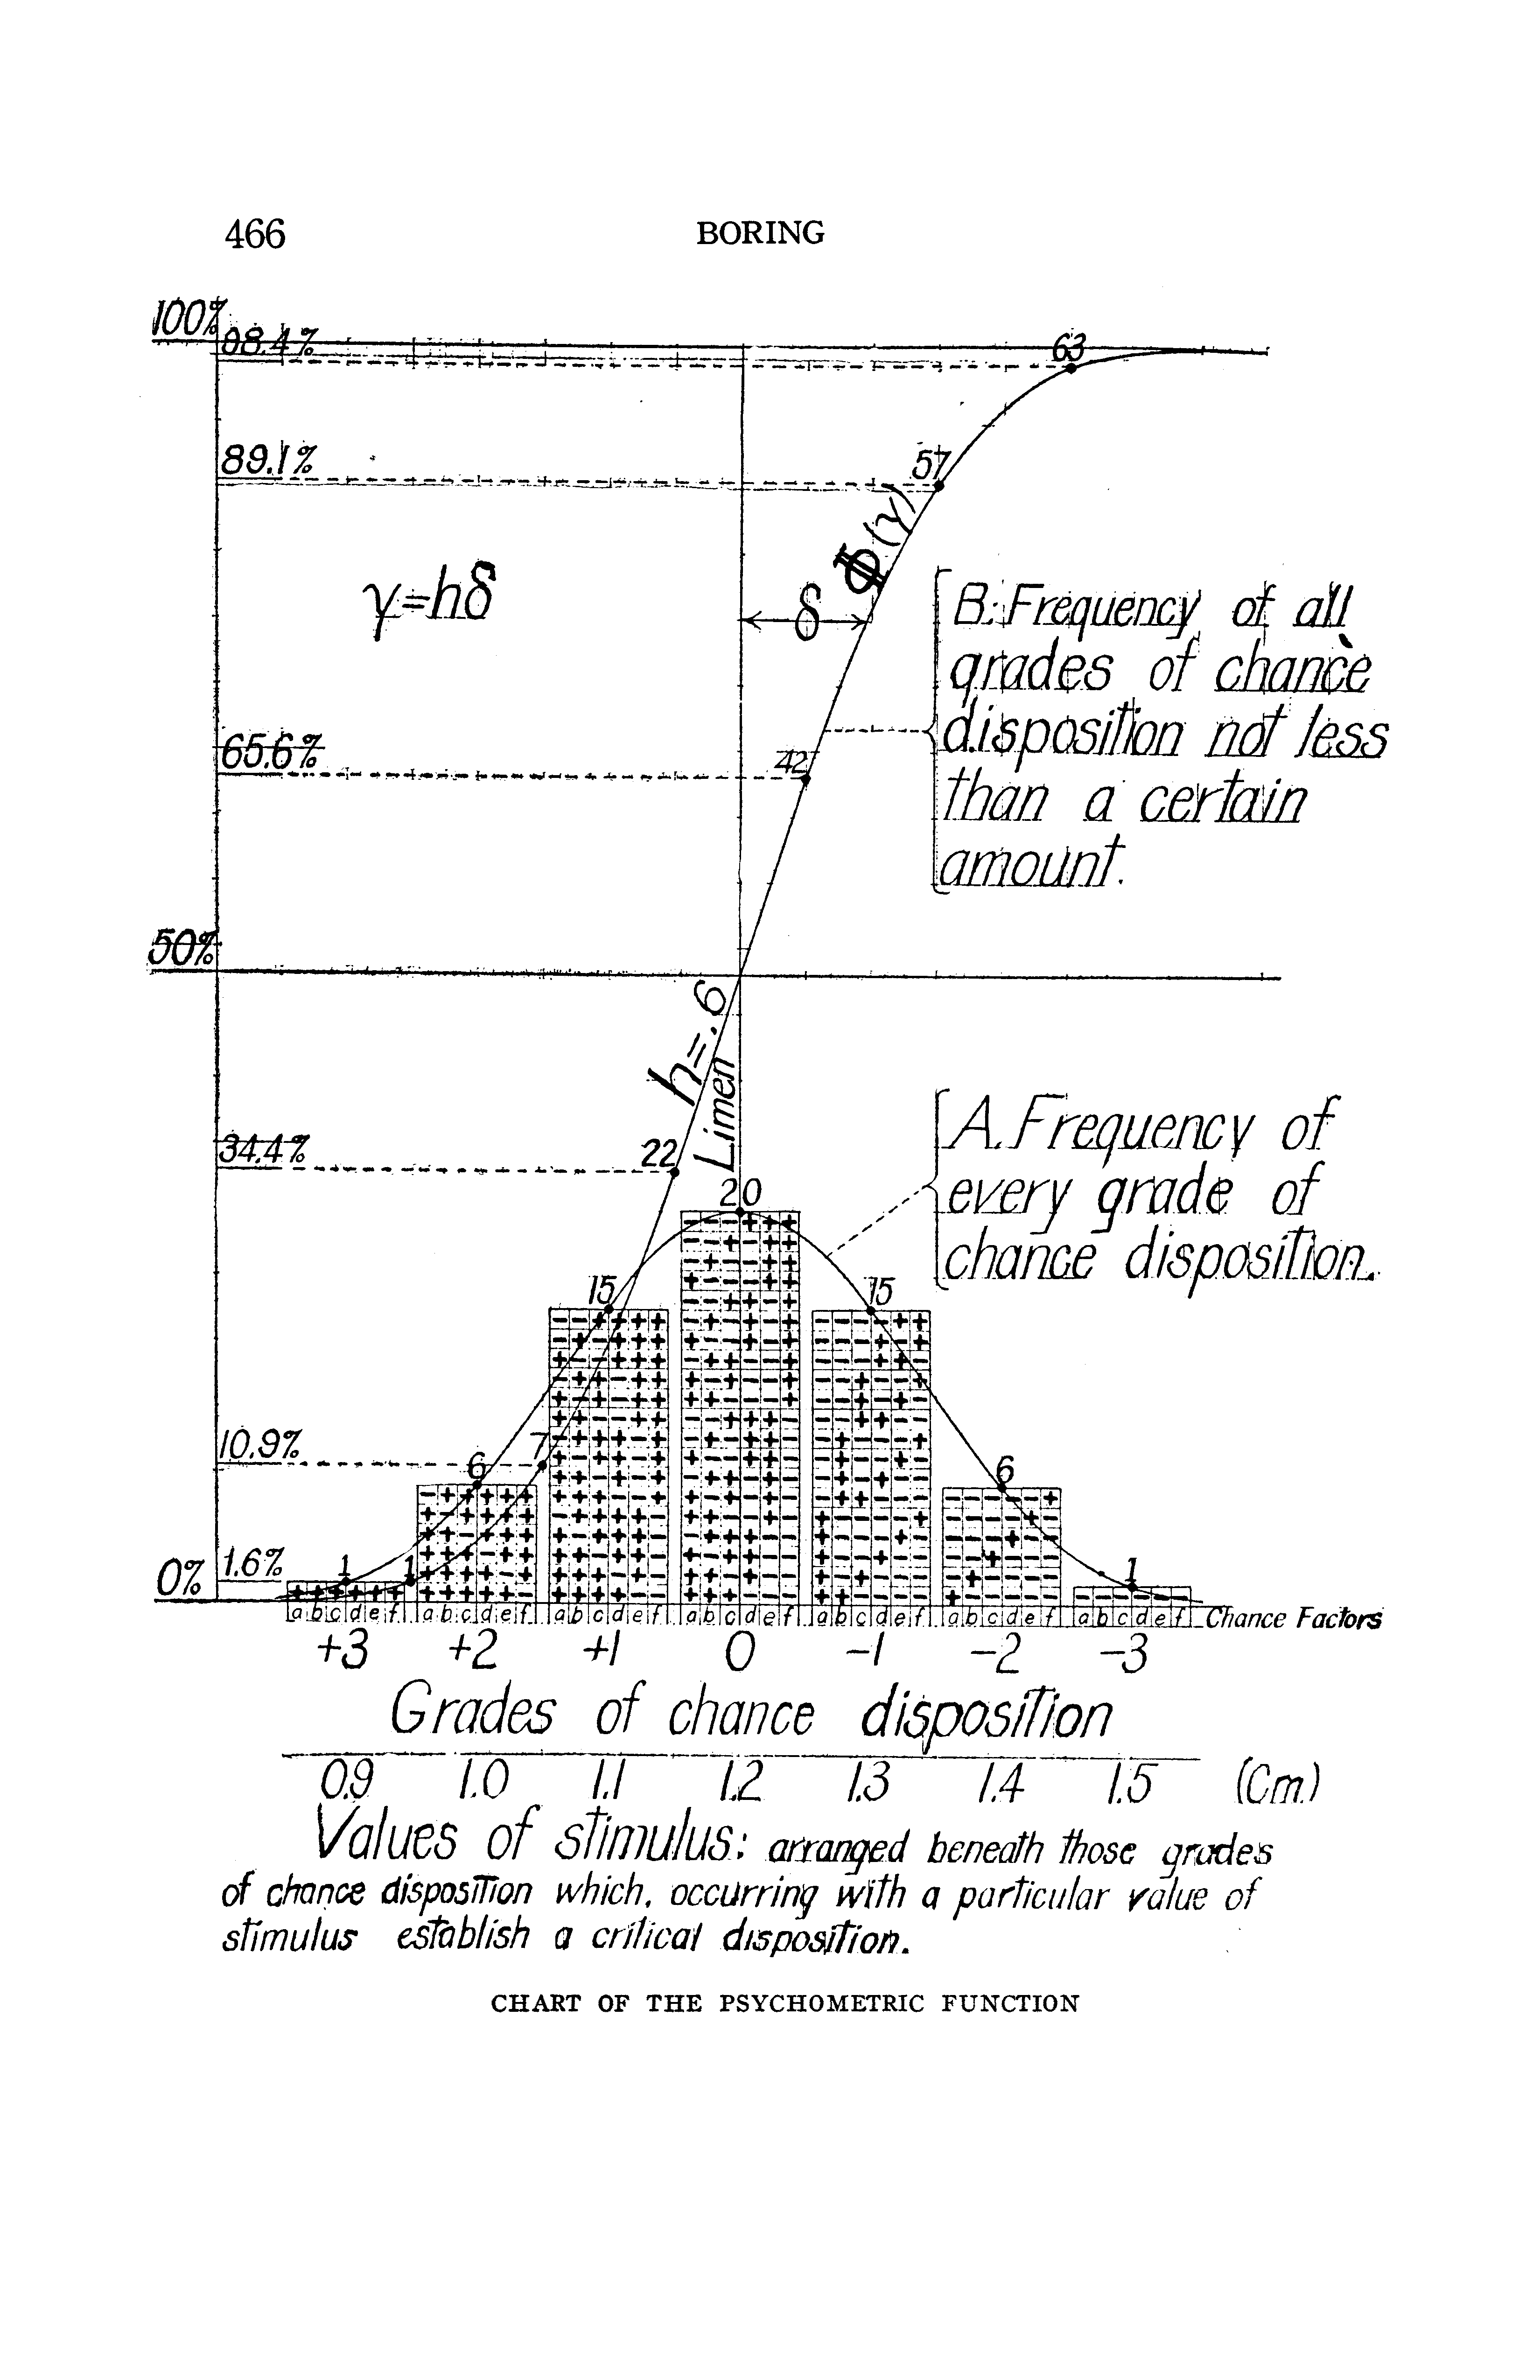
\includegraphics[width=0.7\linewidth]{figures/chart_of_pf} 

}

\caption{A chart of the psychometric function. The experiment in this paper places two points on a subject's skin separated by some distance, and has them answer their impression of whether there is one point or 'two', recorded as either 'two' or 'not two'. As the separation of aesthesiometer points increases, so too does the subject's confidence in their response of 'two'. So at what separation is the impression of two points liminal?}\label{fig:chart-of-pf}
\end{figure}

Figure \ref{fig:chart-of-pf} displays the key aspects of the psychometric function. The most crucial part is the sigmoid function, the S-like non-decreasing curve, which in this case is represented by the Normal CDF, \(\Phi(\gamma)\). The horizontal axis represents the stimulus stimulus intensity, the separation of two points in centimeters. The vertical axis represents the probability that a subject has the impression of two points. With only experimental data, the response proportion becomes an approximation for the probability.

This leads me to talk about the type of psychometric experiment that this paper deals with called a \textbf{temporal order judgment} (TOJ) experiment. The concept is that if there are two distinct stimuli occurring nearly simultaneously then our brains will bind them into a single percept -- perceive them as happening simultaneously. Compensation for small temporal differences is beneficial for coherent multisensory experiences, particularly in visual-speech synthesis as it is necessary to maintain an accurate representation of the sources of multisensory events. The temporal asynchrony between stimuli is called the \textbf{stimulus onset asynchrony} (SOA), and the range of SOAs for which sensory signals are integrated into a global percept is called the \textbf{temporal binding window}. When the SOA grows too large then the brain segregates the two signals and the temporal order can be determined.

Our experiences in life as we age shape the mechanisms of processing multisensory signals, and some multisensory signals are integrated much more readily than others. Perceptual synchrony has been previously studied through the \textbf{point of subjective simultaneity} (PSS) -- the temporal delay between two signals at which an observer is unsure about their temporal order \citep{stone2001now}. The temporal binding window is the time span over which sensory signals arising from different modalities appear integrated into a global percept. A deficit in temporal sensitivity may lead to a widening of the temporal binding window and reduce the ability to segregate unrelated sensory signals. In temporal order judgment tasks, the ability to discriminate the timing of multiple sensory signals is referred to as temporal sensitivity, and is studied through the measurement of the \textbf{just noticeable difference} (JND) -- the smallest lapse in time so that a temporal order can just be determined. Figure \ref{fig:plot-ref-pf} highlights the features through which we study psychometric functions. The PSS is defined as the point where an observer can do no better at determining temporal order than random guessing (i.e.~the response probability is 50\%). The JND is defined as the extra temporal delay between stimuli so that the temporal order is just able to be determined. Historically this has been defined as the difference between the 84\% level and the PSS, though the upper level depends on domain expertise.

\begin{figure}

{\centering 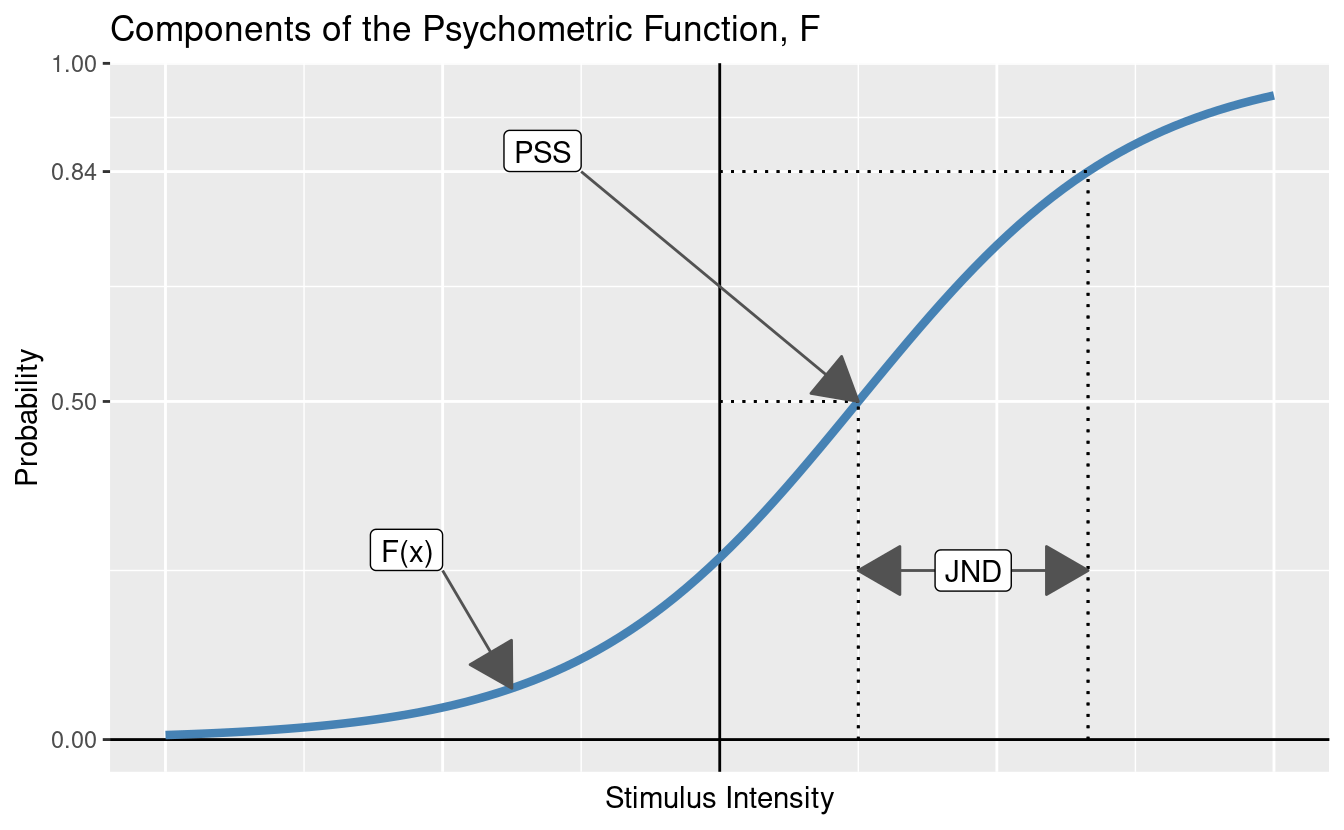
\includegraphics[width=0.7\linewidth]{020-motivating-data_files/figure-latex/plot-ref-pf-1} 

}

\caption{The PSS is defined as the point where an observer can do no better at determining temporal order than random guessing. The just noticeable difference is defined as the extra temporal delay between stimuli so that the temporal order is just able to be determined. Historically this has been defined as the difference between the 0.84 level and the PSS, though the upper level depends on domain expertise.}\label{fig:plot-ref-pf}
\end{figure}

Perceptual synchrony and temporal sensitivity can be modified through a baseline understanding. In order to perceive physical events as simultaneous, our brains must adjust for differences in temporal delays of transmission of both psychical signals and sensory processing \citep{fujisaki2004recalibration}. In some cases such as with audiovisual stimuli, the perception of simultaneity can be modified by repeatedly presenting the audiovisual stimuli at fixed time separations (called an adapter stimulus) to an observer \citep{vroomen2004recalibration}. This repetition of presenting the adapter stimulus is called \textbf{temporal recalibration}.

The data set that I introduce in the next section concerns temporal order judgment across various sensory modalities with a temporal recalibration component.

\hypertarget{toj-task}{%
\section{Temporal Order Judgment Data}\label{toj-task}}

The data set that I am using in this paper comes from experiments done by A.N. Scurry and Dr.~Fang Jiang in the Department of Psychology at the University of Nevada. Reduced temporal sensitivity in the aging population manifests in an impaired ability to perceive synchronous events as simultaneous, and similarly more difficulty in segregating asynchronous sensory signals that belong to different sources. The consequences of a widening of the temporal binding window is considered in \citet{scurry2019aging}, as well as a complete detailing of the experimental setup and recording process. A shortened summary of the methods is provided below.

There are four different tasks in the experiment: audio-visual, visual-visual, visuo-motor, and duration, and I will refer to each task respectively as audiovisual, visual, sensorimotor, and duration. The participants consist of 15 young adults (age 20-27), 15 middle age adults (age 39-50), and 15 older adults (age 65-75), all recruited from the University of Nevada, Reno. Additionally all subjects are right handed and were reported to have normal or corrected to normal hearing and vision.

\begin{table}[!h]

\caption{\label{tab:multitask-data}Sample of motivating data.}
\centering
\begin{tabular}[t]{rrllllrl}
\toprule
soa & response & sid & task & trial & age\_group & age & sex\\
\midrule
-350 & 0 & O-m-BC & audiovisual & pre & older\_adult & 70 & M\\
-200 & 0 & M-m-SJ & duration & post1 & middle\_age & 48 & M\\
28 & 1 & O-f-KK & sensorimotor & pre & older\_adult & 66 & F\\
275 & 1 & O-f-MW & visual & post1 & older\_adult & 69 & F\\
\bottomrule
\end{tabular}
\end{table}

In the audiovisual TOJ task, participants were asked to determine the temporal order between an auditory and visual stimulus. Stimulus onset asynchrony values were selected uniformly between -500 to +500 ms with 50 ms steps, where negative SOAs indicated that the visual stimulus was leading, and positive values indicated that the auditory stimulus was leading. Each SOA value was presented 5 times in random order in the initial block. At the end of each trial the subject was asked to report if the auditory stimulus came before the visual, where a \(1\) indicates that they perceived the sound first, and a \(0\) indicates that they perceived the visual stimulus first.

A similar setup is repeated for the visual, sensorimotor, and duration tasks. The visual task presented two visual stimuli on the left and right side of a display with temporal asynchronies that varied between -300 ms to +300 ms with 25 ms steps. Negative SOAs indicated that the left stimulus was first, and positive that the right came first. A positive response indicates that the subject perceived the right stimulus first. The sensorimotor task has subjects focus on a black cross on a screen. When it disappears, they respond by pressing a button. Additionally, when the cross disappears, a visual stimulus was flashed on the screen, and subjects were asked if they perceived the visual stimulus before or after their button press. The latency of the visual stimulus was partially determined by individual subject's average response time, so SOA values are not fixed between subjects and trials. A positive response indicates that the visual stimulus was perceived after the button press.

The duration task presents two vertically stacked circles on a screen with one appearing right after the other. The top stimulus appeared for a fixed amount of time of 300 ms, and the bottom was displayed for anywhere between +100 ms to +500 ms in 50 ms steps corresponding to SOA values between -200 ms to +200 ms. The subject then responds to if they perceived the bottom circle as appearing longer than the top circle.

\begin{table}[!h]

\caption{\label{tab:toj-summary}Summary of TOJ Tasks}
\centering
\begin{tabular}[t]{lll}
\toprule
Task & Positive Response & Positive SOA Truth\\
\midrule
Audiovisual & Perceived audio first & Audio came before visual\\
Visual & Perceived right first & Right came before left\\
Sensorimotor & Perceived visual first & Visual came before tactile\\
Duration & Perceived bottom as longer & Bottom lasted longer than top\\
\bottomrule
\end{tabular}
\end{table}

Finally, after the first block of each task was completed, the participants went through an adaptation period where they were presented with the respective stimuli from each task repeatedly at fixed temporal delays, then they repeated the task. To ensure that the adaptation affect persisted, the subject were presented with the adapter stimulus at regular intervals throughout the second block. The blocks are designated as \texttt{pre} and \texttt{post1}, \texttt{post2}, etc. in the data set. In this paper I will only be focusing on the \texttt{pre} and \texttt{post1} blocks.

\hypertarget{data-visualizations-and-quirks}{%
\section{Data Visualizations and Quirks}\label{data-visualizations-and-quirks}}

The dependent variable in these experiments is the perceived response which is encoded as a 0 or a 1, and the independent variable is the SOA value. If the response is plotted against the SOA values, then it is difficult to determine any relationship (see figure \ref{fig:simple-response-soa-plot}). Transparency can be used to better visualize the relationships between SOA value and responses. The center plot in figure \ref{fig:simple-response-soa-plot} uses the same data as the left plot, except that the transparency is set to 0.05. As a result, one can see that there is a higher density of ``0'' responses towards more negative SOAs, and a higher density of ``1'' responses for more positive SOAs. Taking it a step further, I can compute and plot the proportion of responses for a given SOA. This is displayed in the right plot. Now the relationship between SOA value and responses is clear -- as the SOA value goes from more negative to more positive, the proportion of positive responses increases from near 0 to near 1.

\begin{figure}

{\centering 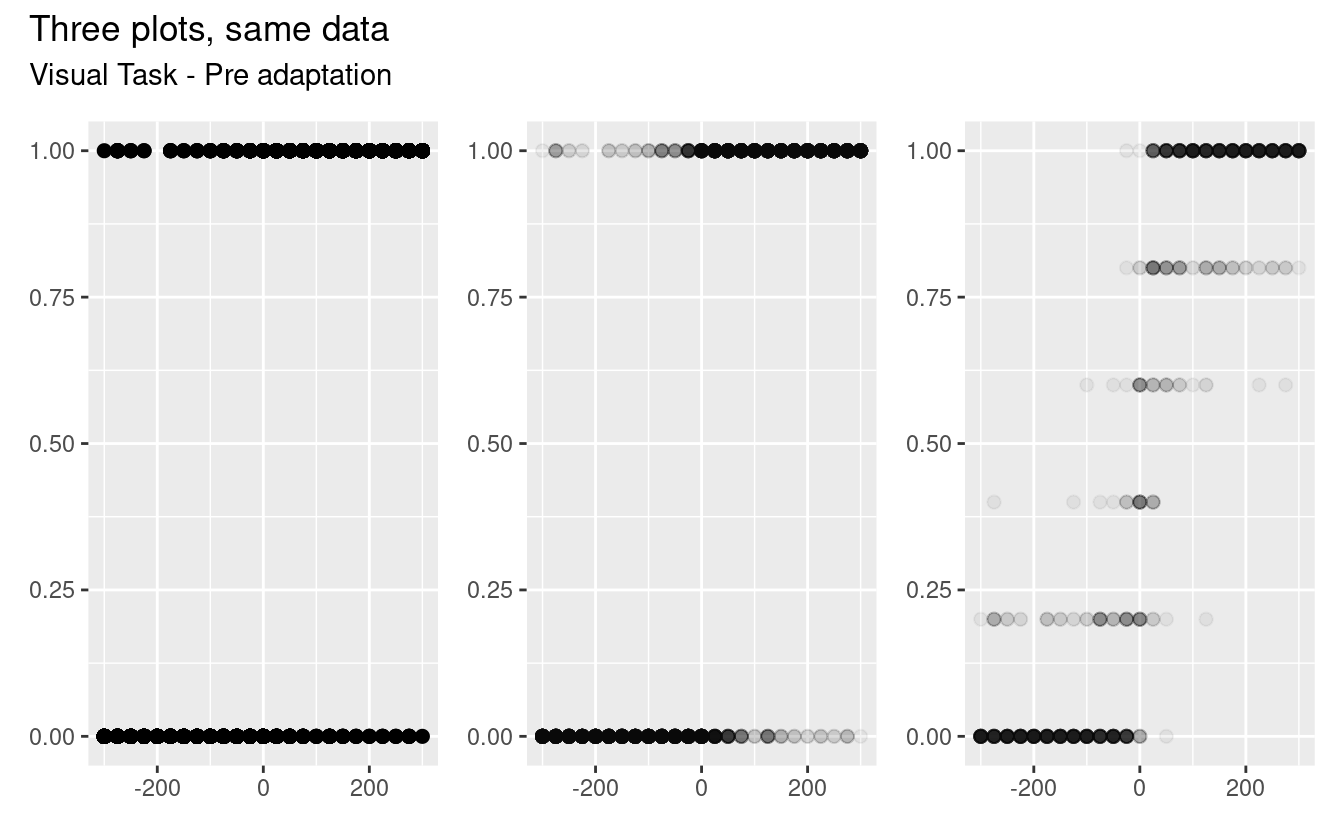
\includegraphics[width=0.7\linewidth]{020-motivating-data_files/figure-latex/simple-response-soa-plot-1} 

}

\caption{Left: Simple plot of response vs. soa value. Center: A plot of response vs. soa with transparency. Right: A plot of proportions vs. soa with transparency.}\label{fig:simple-response-soa-plot}
\end{figure}

Subjectively the right plot in figure \ref{fig:simple-response-soa-plot} is the easiest to interpret. Because of this, I will often present the observed and predicted data using the proportion of responses rather than the actual response. Proportional data also has the advantage of being bounded on the same interval as the response. For the audiovisual task, the responses can be aggregated into binomial data -- the number of positive responses for given SOA value -- which is sometimes more efficient to work with than the Bernoulli data (see table \ref{tab:av-bin-sample}). However the number of times an SOA is presented varies between the pre-adaptation and post-adaptation blocks; 5 and 3 times per SOA respectively.

\begin{table}[!h]

\caption{\label{tab:av-bin-sample}Audiovisual task with aggregated responses.}
\centering
\begin{tabular}[t]{lrrrr}
\toprule
trial & soa & n & k & proportion\\
\midrule
 & 200 & 5 & 4 & 0.80\\
\cmidrule{2-5}
 & 150 & 5 & 5 & 1.00\\
\cmidrule{2-5}
\multirow[t]{-3}{*}{\raggedright\arraybackslash pre} & -350 & 5 & 0 & 0.00\\
\cmidrule{1-5}
 & 350 & 3 & 3 & 1.00\\
\cmidrule{2-5}
 & -500 & 3 & 1 & 0.33\\
\cmidrule{2-5}
\multirow[t]{-3}{*}{\raggedright\arraybackslash post1} & -200 & 3 & 0 & 0.00\\
\bottomrule
\end{tabular}
\end{table}

Other quirks about the data pertain to the subjects. There is one younger subject that did not complete the audiovisual task, and one younger subject that did not complete the duration task. Additionally there is one older subject who's response data for the post-adaptation audiovisual task is unreasonable\footnote{By unreasonable, I mean that it is extremely unlikely that the data represents genuine responses.} (see figure \ref{fig:av-post1-O-f-CE-plot}).

\begin{figure}

{\centering 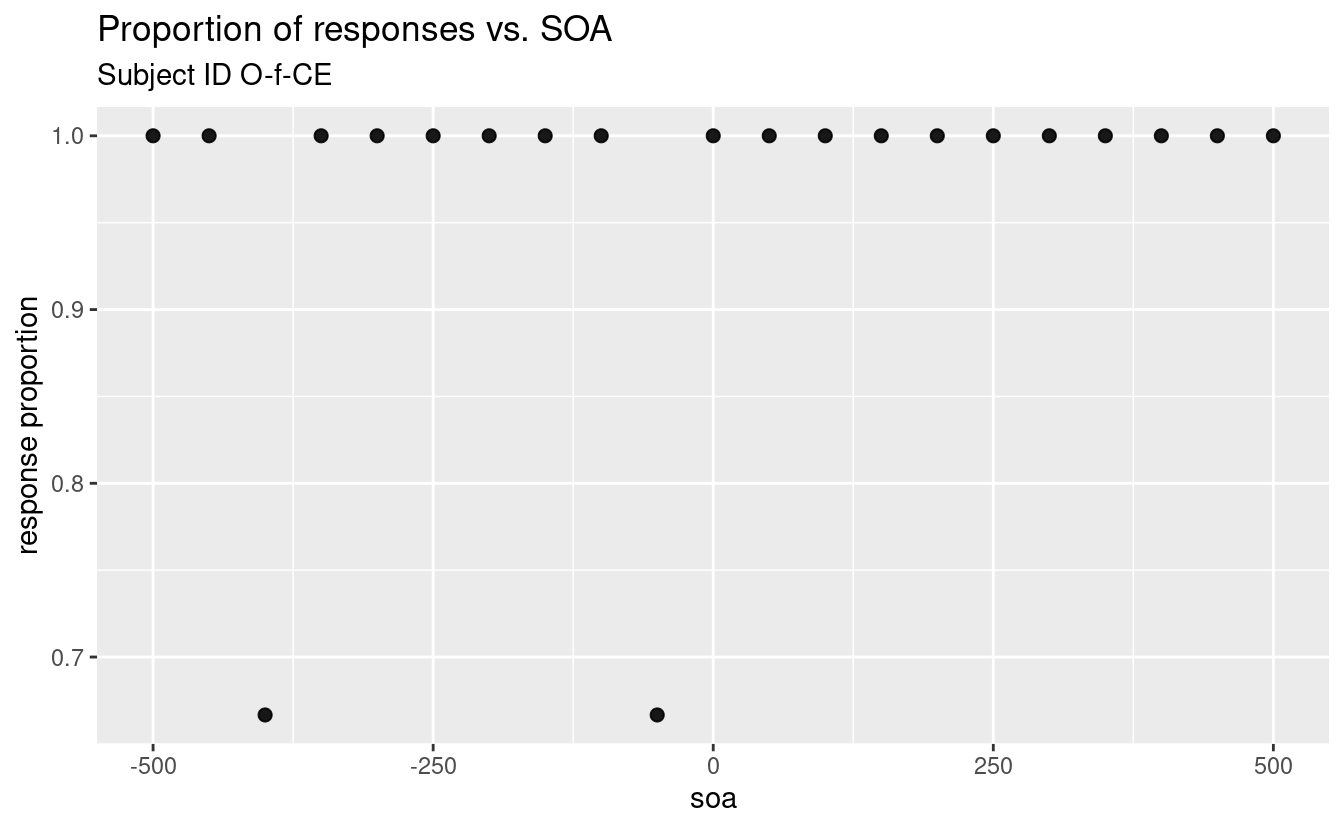
\includegraphics[width=0.7\linewidth]{020-motivating-data_files/figure-latex/av-post1-O-f-CE-plot-1} 

}

\caption{Post-adaptation response data for O-f-CE}\label{fig:av-post1-O-f-CE-plot}
\end{figure}

It is unreasonable because, of all the negative SOAs, there were only two correct responses\footnote{Correct in the sense that the perceived order matches the actual order.}. If a ssubject is randomly guessing the temporal order, then a naive estimate for the proportion of correct responses is 0.5. If a subject's proportion of correct responses is above 0.5, then they are doing better than random guessing. In figure \ref{fig:av-post-neg-trials} it is seen that subject O-f-CE is the only one who's proportion is below 0.5 (and by a considerable amount).

\begin{figure}

{\centering 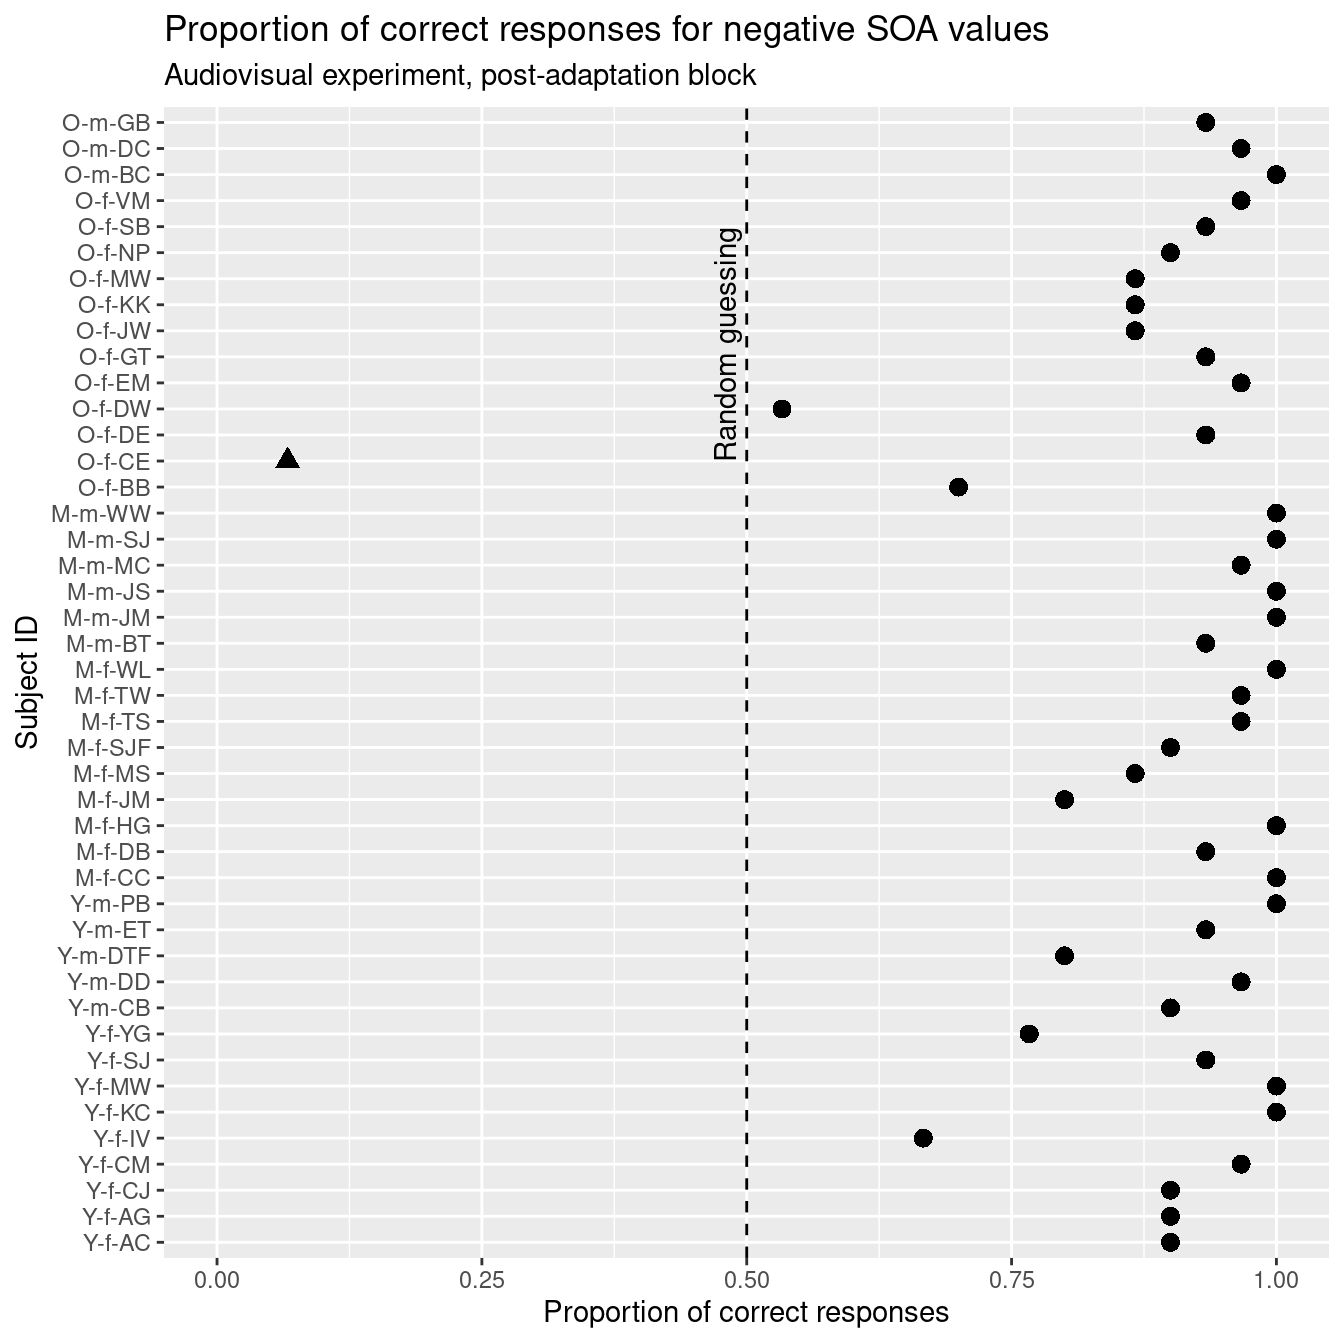
\includegraphics[width=0.7\linewidth]{020-motivating-data_files/figure-latex/av-post-neg-trials-1} 

}

\caption{Proportion of correct responses for negative SOA values during the post-adaptation audiovisual experiment.}\label{fig:av-post-neg-trials}
\end{figure}

The consequences of leaving in this experimental block in the data is considered in the \protect\hyperlink{workflow}{Chapter 5}, but it is a clear outlier that must be noted. When this method of detecting outliers is repeated for all tasks and blocks, then I end up with 17 records in total (see figure \ref{fig:naive-prop-outliers}), one of which is the aforementioned subject.

\begin{figure}

{\centering 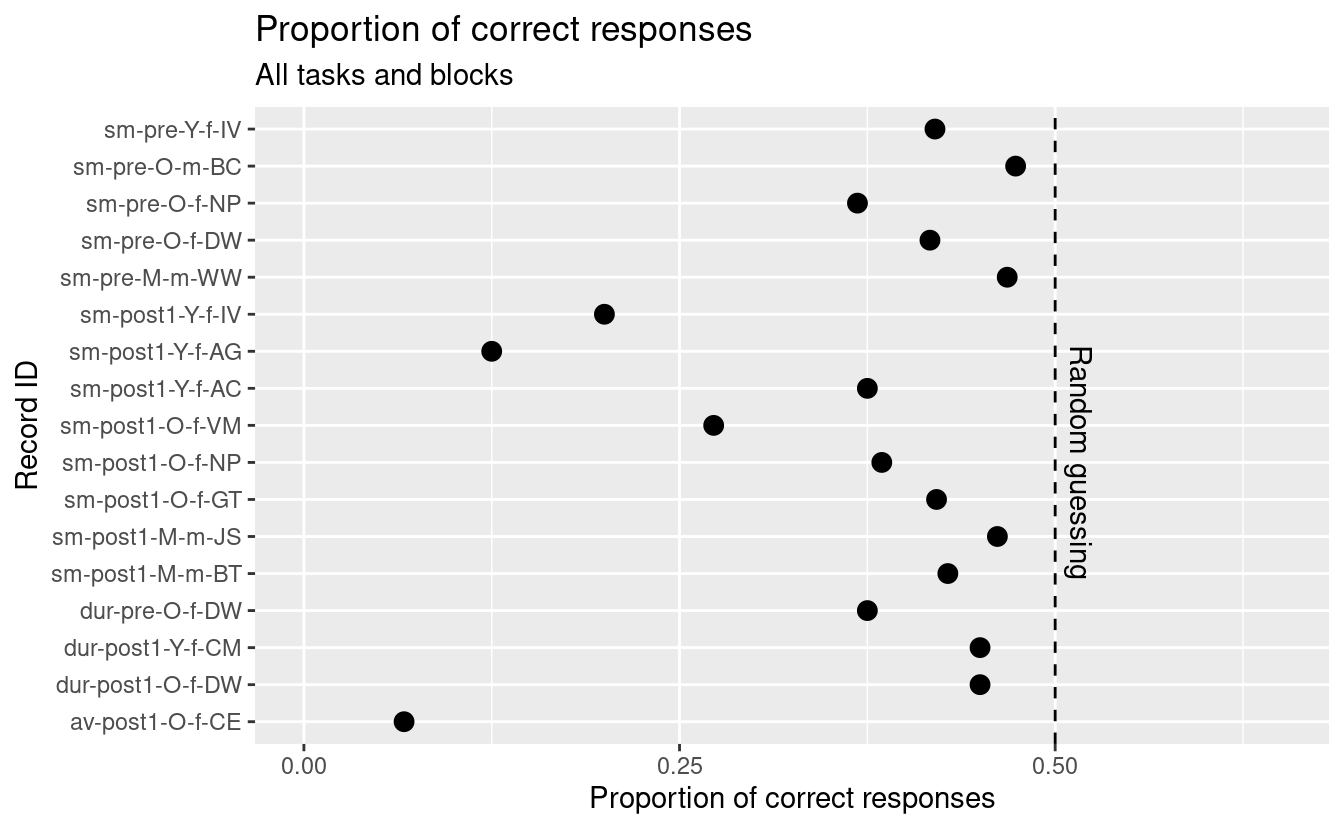
\includegraphics[width=0.7\linewidth]{020-motivating-data_files/figure-latex/naive-prop-outliers-1} 

}

\caption{Proportion of correct responses across all tasks and blocks Proportions are calculated individually for positive and negative SOAs.}\label{fig:naive-prop-outliers}
\end{figure}

Most of the records that are flagged by this method of outlier detection are from the sensorimotor task, and none are from the visual task. This may be caused by the perceived difficulty of the task. One consequence of higher temporal sensitivity is that it is easier to determine temporal order. It may also be that determining temporal order is inherently easier for certain multisensory tasks than others. Since the sensorimotor task does not have fixed SOA values like the other tasks, it may be perceived as more difficult. Or perhaps the mechanisms that process touch and visual signals are not as well coupled as those that process audio and visual signals. I'll consider how to handle the sensorimotor outliers in the model fitting process.

\hypertarget{background}{%
\chapter{Background to Modeling}\label{background}}

A psychometric function can be fit using a generalized linear model (GLM) with the link function coming from the family of S-shaped curves called a sigmoid. Commonly GLMs are fit using maximum likelihood estimation (MLE). In the case of a psychometric experiment, we can represent the outcome of a single trial as the result of a random experiment arising from a Bernoulli process. Without loss of generality, the psychometric function, \(F(x; \theta)\), determines the probability that the outcome is 1.

\begin{align*}
Y &\sim \textrm{Bernoulli}(\pi) \\
\pi &= P(Y=1 \vert x; \theta) = F(x; \theta)
\end{align*}

If \(P(Y=1 | x; \theta) = F(x;\theta)\), then \(P(Y = 0 | x; \theta) = 1 - F(x;\theta)\), and hence the probability of an outcome is

\begin{equation}
  P(Y=y | x; \theta) = F(x;\theta)^y(1-F(x;\theta))^{1-y}
  \label{eq:bernproby}
\end{equation}

The likelihood function, \(\mathcal{L}\), can be determined using equation \eqref{eq:bernproby}

\begin{equation}
  \begin{split}
    \mathcal{L}(\theta | y, x) &= \prod_{i}^{N} P(y_i | x_i; \theta) \\
    &= \prod_{i}^{N}F(x_i;\theta)^{y_i}(1-F(x_i;\theta))^{1-y_i}
  \end{split}
  \label{eq:bernlik}
\end{equation}

Equation \eqref{eq:bernlik} is commonly expressed in terms of its logarithm.

\begin{equation}
  \ln \mathcal{L}(\theta | y, x) = \sum_{i}^{N} y_i \ln\left(F(x_i;\theta)\right) + (1-y_i) \ln\left(F(x_i;\theta))\right)
  \label{eq:bernloglik}
\end{equation}

From here the classical approach would be to take the derivative of \eqref{eq:bernloglik}, set it equal to \(0\), and solve for \(\theta\). Additionally one might perform a second derivative test to ensure that the solution is indeed a maximizer to \eqref{eq:bernloglik} (and hence to \eqref{eq:bernlik}). However no closed form expression exists for the solution to \(\frac{d}{d\theta} \ln \mathcal{L}(\theta) = 0\), and so numerical optimization methods like gradient descent are used to iteratively find the MLE solution. In most cases this works fine, but there are common situations where MLE fails. In this chapter I will discuss common techniques for fitting psychometric functions, the reasons to use these methods, and the conditions for when they are not optimal.

As introduced above, the first method is to use generalized linear models. A GLM is one that can be transformed into a linear model via a link function. An example of this is the logistic function which takes \(x \in \mathbb{R}\) and squishes the output to be in \((0, 1)\).

\begin{equation}
  F(\theta) = \frac{1}{1 + \exp\left(-\theta\right)}
  \label{eq:logistic}
\end{equation}

Since \(F\) is a strictly increasing and continuous function, it has an inverse, and the link for \eqref{eq:logistic} is the log-odds or logit function.

\begin{equation}
  F^{-1}(\pi) = \mathrm{logit}(\pi) = \ln\left(\frac{\pi}{1 - \pi}\right)
  \label{eq:logit}
\end{equation}

By taking \((F^{-1} \circ F)(\theta)\) we can arrive at a relationship that is linear in \(\theta\).

\begin{align*}
  \pi = F(\theta) \Longleftrightarrow F^{-1}(\pi) &= F^{-1}(F(\theta)) \\
  & = \ln\left(\frac{F(\theta)}{1 - F(\theta)}\right) \\
  &= \ln(F(\theta)) - \ln(1 - F(\theta)) \\
  &= \ln\left(\frac{1}{1 + \exp(-\theta)}\right) - \ln\left(\frac{\exp(-\theta)}{1 + \exp(-\theta)}\right) \\
  &= - \ln(1 + \exp(-\theta)) - \ln(\exp(-\theta)) + \ln(1 + \exp(-\theta)) \\
  &= - \ln(\exp(-\theta)) \\
  &= \theta
\end{align*}

Linear models are favored in statistics because they are generally easier to interpret than other types of models. For example, say \(\mathrm{logit}(\pi) = 0.5 + 1.5x\) where \(\pi\) is the probability of a positive outcome, \(Y=1\). We can say that at \(x = 0\), the log-odds of a positive outcome is 0.5, and an increase in \(x\) by 1 increases the log-odds by 1.5.

There is nothing that is particular about the logistic function that makes it the only suitable sigmoid for psychometric functions. Other common link functions include the probit (inverse of the standard normal CDF) and Weibull inverse CDF. In fact, any continuous CDF defined on the real number line can be used for psychometric functions. A PF only requires that a function is strictly increasing and bounded between 0 and 1.The logit and probit links have properties such as connections to log-odds and the normal distribution that make working with them more convenient.

\begin{itemize}
\tightlist
\item
  Generalized Linear Models

  \begin{itemize}
  \tightlist
  \item
    classical approaches to fitting/estimation

    \begin{itemize}
    \tightlist
    \item
      Maximum likelihood estimation

      \begin{itemize}
      \tightlist
      \item
        Simple and almost every piece of statistical software will have an implementation
      \end{itemize}
    \end{itemize}
  \item
    Expectation Maximization
  \item
    Random effects (Gelmen and Hill)
  \item
    Bayesian GLMs

    \begin{itemize}
    \tightlist
    \item
      Completely reliant on MCMC
    \end{itemize}
  \end{itemize}
\item
  Model-free estimations (footnote? remark?)

  \begin{itemize}
  \tightlist
  \item
    non-parametric models
  \item
    \citep{zchaluk2009model}
  \end{itemize}
\item
  Bayesian logistic regression

  \begin{itemize}
  \tightlist
  \item
    \citet{gelman2008weakly}
  \item
    Can't completely express the structure (hierarchy) of the data
  \end{itemize}
\item
  Residual Analysis

  \begin{itemize}
  \item
    using the fitted values vs.~the observed values to evaluate goodness of fit
  \item
  \end{itemize}
\item
  So what's the answer?

  \begin{itemize}
  \tightlist
  \item
    The last two options (bayes + multilevel) when on their own do well, but are not robust to
  \end{itemize}
\item
  shortcomings

  \begin{itemize}
  \tightlist
  \item
    Convergence failure in the presence of complete separation

    \begin{itemize}
    \tightlist
    \item
      \citep{prins2019too}, \citep{ghosh2018use}
    \item
      Give an example with how the MLE values are estimated
    \item
      Give an example where MLE fails
    \end{itemize}
  \end{itemize}
\end{itemize}

\hypertarget{bayesian-modeling}{%
\chapter{Bayesian Multilevel Modeling}\label{bayesian-modeling}}

\begin{itemize}
\tightlist
\item
  short intro

  \begin{itemize}
  \tightlist
  \item
    sentence 1
  \item
    sentence 2
  \item
    sentence 3
  \end{itemize}
\end{itemize}

\hypertarget{bayesian-stuff}{%
\section{Bayesian Stuff}\label{bayesian-stuff}}

\begin{itemize}
\item
  Mathematical foundations

  \begin{itemize}
  \tightlist
  \item
    Bayes rule in regression setting
  \end{itemize}
\item
  Easy in theory, difficult in practice

  \begin{itemize}
  \tightlist
  \item
    Example of a conjugate priors
  \item
    need more complexity -\textgreater{} computer methods
  \item
    Computer methods needed
  \end{itemize}
\item
\end{itemize}

\hypertarget{multilevel-modeling-stuff}{%
\section{Multilevel Modeling Stuff}\label{multilevel-modeling-stuff}}

\begin{itemize}
\item
  Estimating the variance at different levels in the model
\item
\end{itemize}

\hypertarget{workflow}{%
\chapter{Principled Bayesian Workflow}\label{workflow}}

There are many great resources out there\footnote{citation needed} for following along with an analysis of some data or problem, and much more is the abundance of tips, tricks, techniques, and testimonies to good modeling practices. The problem is that many of these prescriptions are given without context for when they are appropriate to be taken. According to \citet{betancourt2020}, this leaves ``practitioners to piece together their own model building workflows from potentially incomplete or even inconsistent heuristics.'' The concept of a principled workflow is that for any given problem, there is not, nor should there be, a default set of steps to take to get from data exploration to predictive inferences. Rather great consideration must be given to domain expertise and the questions that one is trying to answer with the data.

Since everyone asks different questions, the value of a model is not in how well it ticks the boxes of goodness-of-fit checks, but in consistent it is with domain expertise and its ability to answer the unique set of questions. Betancourt suggests answering four questions to evaluate a model by:

\begin{enumerate}
\def\labelenumi{\arabic{enumi}.}
\tightlist
\item
  Domain Expertise Consistency - Is our model consistent with our domain expertise?
\item
  Computational Faithfulness - Will our computational tools be sufficient to accurately fit our posteriors?
\item
  Inferential Adequacy - Will our inferences provide enough information to answer our questions?
\item
  Model Adequacy - Is our model rich enough to capture the relevant structure of the true data generating process?
\end{enumerate}

\begin{itemize}
\tightlist
\item
  Scope out your problem
\item
  Specify likelihood and priors
\item
  check the model with fake data
\item
  fit the model to the real data
\item
  check diagnostics
\item
  graph fit estimates
\item
  check predictive posterior
\item
  compare models
\end{itemize}

\hypertarget{iteration-1-the-journey-of-a-thousand-miles-begins-with-a-single-step}{%
\section{Iteration 1 (The Journey of a Thousand Miles Begins with a Single Step)}\label{iteration-1-the-journey-of-a-thousand-miles-begins-with-a-single-step}}

\hypertarget{pre-model-pre-data}{%
\subsection{Pre-Model, Pre-Data}\label{pre-model-pre-data}}

We begin the modeling process by modeling the experiment according to the description of how it occurred and how the data were collected. This first part consists of conceptual analysis, defining the observational space, and constructing summary statistics that can help us to identify issues in the model specification.

\hypertarget{conceptual-analysis}{%
\subsubsection{Conceptual analysis}\label{conceptual-analysis}}

In section \ref{toj-task} we discussed the experimental setup and data collection. To reiterate, subjects are presented with two stimuli separated by some temporal delay, and they are asked to respond as to their perception of the temporal order. There are 45 subjects with 15 each in the young, middle, and older age groups. As the SOA becomes larger in the positive direction, we expect subjects to give more ``positive'' responses, and as the SOA becomes larger in the negative direction, we expect more ``negative'' responses. By the way the experiment and responses are constructed, we would not expect to see a reversal of this trend unless there was an issue with the subject's understanding of the directions given to them or an error in the recording device.

We also know that after the first experimental block the subjects go through a recalibration period, and repeat the experiment again. We are interested in seeing if the recalibration has an effect on temporal sensitivity and perceptual synchrony, and if the effect is different for each age group.

\hypertarget{define-observational-space}{%
\subsubsection{Define observational space}\label{define-observational-space}}

The response that subjects give to a TOJ task is recorded as a zero or a one (see section \ref{toj-task}), and their relative performance is determined by the SOA value. Let \(y\) represent the binary outcome of a trial and let \(x\) be the SOA value.

\begin{align*}
y_i &\in \lbrace 0, 1\rbrace \\
x_i &\in \mathbb{R}
\end{align*}

If the SOA values are fixed like in the audiovisual task, then the responses can be aggregated into binomial counts, \(k\).

\[
k_i, n_i \in \mathbb{Z}_0^+, k_i \le n_i
\]

In the above equation, \(\mathbb{Z}_0^+\) represents the set of non-negative integers. Notice that the number of trials \(n\) has an index variable \(i\). This is because the number of trials per SOA is not fixed between blocks. In the pre-adaptation block, there are five trials per SOA compared to three in the post-adaptation block. So if observation 32 is recorder during a ``pre'' block, \(n_{32} = 5\), and if observation 1156 is during a ``post'' block, \(n_{1156} = 3\).

Then we also have the three categorical variables -- age group, subject ID, and adaptation. For the first two, we treat them as factor variables\footnote{Factor variables also go by the name index variable or categorical variable}. Rather than using one-hot encoding or dummy variables, we leave the age levels as categories and fit a coefficient for each level. Among the benefits of this approach is the ease of interpretation and ease of working with the data programmatically. This is especially true at the subject level. If we used dummy variables for all 45 subjects, we would have 44 different dummy variables to work with, times the number of coefficients that make estimates at the subject level. In the final iteration of our model, this can be as many as \(44 \times 4 = 176\) dummy variables for the subject level!

Age groups and individual subjects can be indexed in the same way that we index the number of trials. \(S_i\) refers to the subject in record \(i\), and similarly \(G_i\) refers to the age group of that subject. Observation 63 is for record ID av-post1-M-f-HG, so then \(S_{63}\) is M-f-HG and \(G_{63}\) is middle\_age. Under the hood of R, these factor levels are represented as integers (e.g.~middle age group level is stored internally as the number 2).

We treat the pre- and post-adaptation categories as a binary indicator referred to as \(trt\) (short for treatment) since there are only two levels in the category. In this setup, a value of 1 indicates a post-adaptation block. We chose this encoding over the reverse because the pre-adaptation block is like the baseline performance, and it seemed more appropriate to interpret the post-adaptation block as turning on some effect. Using a binary indicator in a regression setting may not be the best practice as we discuss in section \ref{mod-dev-iter2}.

We will be using the Stan probabilistic programming language to estimate the model for our data. In the Stan modeling language, data for a binomial model with subject and age group levels and treatment is specified as

\begin{verbatim}
data {
  int N;        // Number of observations
  int N_S;      // Number of subject levels
  int N_G;      // Number of age group levels
  int N_T;      // Number of treatment/control groups
  int n[N];     // Trials per SOA
  int k[N];     // binomial counts
  vector[N] x;  // SOA values
  int S[N];     // Subject identifier
  int G[N];     // Age group identifier
  int trt[N];   // Treatment indicator
}
\end{verbatim}

However, in most of this paper we will be using the \texttt{rethinking} package \citep{R-rethinking} which is a high level wrapper around \texttt{rstan}. For most of the model fitting and analyses, it is sufficient. For more complex routines and for finer control, we will utilize \texttt{rstan} directly.

\hypertarget{construct-summary-statistics}{%
\subsubsection{Construct summary statistics}\label{construct-summary-statistics}}

In order to effectively challenge the validity of our model, we construct a set of summary statistics that help answer the questions of domain expertise consistency and model adequacy. We are studying the affects of age and temporal recalibration through the PSS and JND (see section \ref{psycho-experiments}), so it is natural to define summary statistics around these quantities to verify model consistency. Additionally the PSS and JND can be computed regardless of the model parameterization or chosen psychometric function.

By the experimental setup and recording process, it is impossible that a properly conducted block would result in a JND less than 0 (i.e.~the psychometric function is always non-decreasing), so that can be a lower limit for its threshold. On the other end it is unlikely that it will be beyond the limits of the SOA values, but even more concrete, it seems unlikely (though not impossible) that the just noticeable difference would be more than a second.

A histogram of computed PSS and JND values will suffice for summary statistics. We can estimate the proportion of values that fall outside of our limits defined above, and use them as indications of problems with the model fitting or our conceptual understanding.

\hypertarget{post-model-pre-data}{%
\subsection{Post-Model, Pre-Data}\label{post-model-pre-data}}

We will now define priors for our model, still not having looked at the data. The priors should be motivated by domain expertise and \emph{prior knowledge}, not the data.

\hypertarget{model-development}{%
\subsubsection{Model development}\label{model-development}}

Talk here about linear parameterization and connection to PSS and JND.

Talk here about how I select priors for the intercept (PSS) and the slope (JND). Choose a standard deviation for intercept so that \(\approx 95\%\) of the values are between \(\pm 0.1\)

\begin{align*}
\alpha &\sim \mathcal{N}(0, 0.05) \\
\beta &\sim \mathrm{Lognormal}(3.96, 1.2)
\end{align*}

If the expected JND is 0.100 (100 ms) and is distributed log-normally, then \(\mathrm{logit}(0.84)/jnd\) is also log-normally distributed with mean \(\mathrm{logit}(0.84) - log(0.1) \approx 3.96\).

Choose a standard deviation value so that \(\approx 99\%\) of the JND values are less than 1.

The distribution of prior psychometric functions now looks like

Notice that the family of psychometric functions covers the broad range of possible slopes and intercepts, though the prior distribution appears to put more weight on steeper slopes (smaller JNDs). There is also too much possibility that the PF is nearly flat. We can reduce the mean-log and sd-log of the slope parameter and get a much more uniform-looking distribution of prior psychometric curves.

\begin{align*}
\alpha &\sim \mathcal{N}(0, 0.05) \\
\beta &\sim \mathrm{Lognormal}(3.0, 1.5)
\end{align*}

This prior distribution is much more reasonable. There is good prior coverage of both very steep slopes and very shallow slopes, but not so wide that nearly flat or nearly vertical slopes are likely. Also notice how the spread around \(y=0.5\) remains the same independent of the slope values. This is because of how the model is parameterized. If instead we parameterized the linear predictor as

\[
\mathrm{logit}(\pi) = \alpha^* + \beta^* \times x
\]

then the PSS would depend on both \(\alpha^*\) and \(\beta^*\)

\[
\mathrm{PSS}^* = -\frac{\alpha^*}{\beta^*}
\]

while the JND would remain the same

\[
\mathrm{JND}^* = \mathrm{logit}(0.84)/\beta^*
\]

The problem is that it is much harder to define priors for the slope and intercept when they are so closely coupled, and the interpretation of the parameters becomes more difficult as well.

We can now extend the Stan program to include the parameters and model.

\begin{verbatim}
parameters {
  real alpha;          // Intercept (PSS)
  real<lower=0> beta;  // Slope (logit(0.84) / JND)
}
model {
  alpha ~ normal(0, 0.05);      // Prior for intercept
  beta ~ lognormal(3.0, 1.5);   // Prior for slope
  vector[N] p;                  // Binomial probability
  for (i in 1:N) {
    p[i] = beta * (x[i] - alpha);
  }
  k ~ binomial_logit(n, p); // Observational model
}
\end{verbatim}

\hypertarget{construct-summary-functions}{%
\subsubsection{Construct summary functions}\label{construct-summary-functions}}

NA

\hypertarget{simulate-bayesian-ensemble}{%
\subsubsection{Simulate bayesian ensemble}\label{simulate-bayesian-ensemble}}

What is the purpose of this step? To make sure that the generating model coupled with the summary stats/functions yields prior estimates that are consistent with domain expertise (see \ref{prior-checks}).

\hypertarget{prior-checks}{%
\subsubsection{Prior checks}\label{prior-checks}}

\begin{quote}
If the prior predictive checks indicate con ict between the model and our domain expertise then we have to return to step four {[}(model development){]} and refine our model.
\end{quote}

We're satisfied with the prior coverage of the PSS and JND, so now we can move on to fitting the model to the simulated data.

\hypertarget{configure-algorithm}{%
\subsubsection{Configure algorithm}\label{configure-algorithm}}

As a default, we will be using the \texttt{rstan} package \citep{R-rstan}.

\hypertarget{fit-simulated-ensemble}{%
\subsubsection{Fit simulated ensemble}\label{fit-simulated-ensemble}}

\hypertarget{algorithmic-calibration}{%
\subsubsection{Algorithmic calibration}\label{algorithmic-calibration}}

Did the algorithm perform correctly? What kind of diagnostics exist for this algorithm?

\begin{itemize}
\tightlist
\item
  Using HMC

  \begin{itemize}
  \tightlist
  \item
    \(\hat{R}\)
  \item
    Divergences
  \item
    Effective sample size
  \item
    Tail effective sample size
  \item
    Bulk effective sample size
  \item
    Bayesian fraction of missing information
  \end{itemize}
\end{itemize}

Is there anything we can tune during the fitting process that can alleviate algorithmic issues? Or is it a case of Folk Theorem, and we need to adjust the model?

\hypertarget{inferential-calibration}{%
\subsubsection{Inferential calibration}\label{inferential-calibration}}

Non-identifiable model??

\begin{quote}
In either case we might have to return to Step One to consider an improved experimental design or tempered scientific goals. Sometimes we may only need to return to Step Four to incorporate additional domain expertise to improve our inferences.
\end{quote}

\hypertarget{post-model-post-data}{%
\subsection{Post-Model, Post-Data}\label{post-model-post-data}}

\hypertarget{fit-observation}{%
\subsubsection{Fit observation}\label{fit-observation}}

\hypertarget{diagnose-posterior-fit}{%
\subsubsection{Diagnose posterior fit}\label{diagnose-posterior-fit}}

\begin{quote}
If any diagnostics indicate poor performance then not only is our computational method suspect but also our model might not be rich enough to capture the relevant details of the observed data. At the very least we should return to Step Eight and enhance our computational method.
\end{quote}

\hypertarget{posterior-retrodictive-checks}{%
\subsubsection{Posterior retrodictive checks}\label{posterior-retrodictive-checks}}

Need an example of using summary stats on posterior retrodictions

Oh no! The posterior retrodictions have failed to capture the variation in the observed data. Even though there were no problems in the model fitting process, we did not come up with a model that is complex enough to capture the features of the data. Of course, we intentionally left out the treatment, age group, and subject variables in order to create a baseline model that we can build off of. We will now go through a second iteration of the model starting back at step 4: model development.

\hypertarget{iteration-2-electric-boogaloo}{%
\section{Iteration 2 (Electric Boogaloo)}\label{iteration-2-electric-boogaloo}}

\hypertarget{mod-dev-iter2}{%
\subsection{Model Development}\label{mod-dev-iter2}}

In this iteration we will now add in the treatment and age group levels. Instead of modeling the prior distribution of the slope as log-normal, we model it as a normal distribution and then take the exponential. This allows us to also model the age group and treatment slopes as normally distributed and with an additive affect.

\begin{align*}
\beta &\sim \mathcal{N}(2.5, 1^2) \\
\beta_G &\sim \mathcal{N}(0, \sigma_{\beta G}^2) \\
\beta_T &\sim \mathcal{N}(0, 1^2) \\
\beta_{TG} &\sim \mathcal{N}(0, \sigma_{\beta TG}^2) \\
\mu_\beta &\sim \exp(\beta + \beta_G + (\beta_T + \beta_{TG})\times trt)
\end{align*}

In the above formulation, \(\mu_\beta\) is a log-normal random variable with mean-log \(2.5\) and variance-log \(1^2 + \sigma_{\beta G}^2\) if it's the pre-adaptation block, and \(\left(\sqrt{1^2 + 1^2}\right)^2 + \sigma_{\beta G}^2 + \sigma_{\beta TG}^2\) if it's the post-adaptation block. Values that are negative reduce the slope (increase the JND), and values that are positive increase the slope (reduce the JND).

But wait! this model implies that there is more uncertainty about the post-adaptation trials compared to the baseline trials, and this is not necessarily true. Furthermore, as we'll see in the linear part of model, the intercept, \(\alpha\), is no longer the average response probability of the sample, but is instead exclusively the average for the pre-adaptation trials. This may not matter in certain analyses, but one nice property of multilevel models is the separation of population level estimates and group level estimates. So we modify the model for the slope to be:

\begin{align*}
\beta &\sim \mathcal{N}(2.5, 1^2) \\
\beta_G &\sim \mathcal{N}(0, \sigma_{\beta G}^2) \\
\beta_T &\sim \mathcal{N}(0, \sigma_{\beta T}^2) \\
\mu_\beta &= \exp(\beta + \beta_G + \beta_T)
\end{align*}

Now \(\mu_\beta\) is a log-normal random variable with mean-log \(2.5\) and variance-log \(1^2 + \sigma_{\beta G}^2 + \sigma_{\beta T}^2\), regardless of whether it's the pre-adaptation or the post-adaptation block.

The intercept term can be specified similarly. Conservatively we choose the prior for the intercepts to be normally distributed with mean 0.

\begin{align*}
\alpha &\sim \mathcal{N}(0, 0.05^2) \\
\alpha_G &\sim \mathcal{N}(0, \sigma_{\alpha G}^2) \\
\alpha_T &\sim \mathcal{N}(0, \sigma_{\alpha T}^2) \\
\mu_\alpha &= \alpha + \alpha_{G} + \alpha_{T}
\end{align*}

The parameters and model of the Stan program is

\begin{verbatim}
parameters {
  real a;
  real aG[N_G];
  real aT[N_T];
  
  real b;
  real bG[N_G];
  real bT[N_T];
  
  real<lower=machine_precision()> sd_aG;
  real<lower=machine_precision()> sd_aT;
  real<lower=machine_precision()> sd_bG;
  real<lower=machine_precision()> sd_bT;
}
model {
  a ~ normal(0, 0.05);
  aG ~ normal(0, sd_aG);
  aT ~ normal(0, sd_aT);
  
  b ~ normal(2.5, 1.0);
  bG ~ normal(0, sd_bG);
  bT ~ normal(0, sd_bT);
  
  sd_aG ~ cauchy(0, 0.05);
  sd_aT ~ cauchy(0, 0.05);
  sd_bG ~ cauchy(0, 0.5);
  sd_bT ~ cauchy(0, 0.5);
  
  vector[N] p;
  for (i in 1:N) {
    real mu_b = exp(b + bG[G[i]] + bT[T[i]]);
    real mu_a = a + aG[G[i]] + aT[T[i]];
    p[i] = mu_b * (x[i] - mu_a);
  }
  k ~ binomial_logit(n, p); // Observational model
}
\end{verbatim}

\hypertarget{simulate-bayesian-ensemble}{%
\subsection{Simulate bayesian ensemble}\label{simulate-bayesian-ensemble}}

\hypertarget{prior-checks}{%
\subsection{Prior Checks}\label{prior-checks}}

\hypertarget{configure-algorithm}{%
\subsection{Configure algorithm}\label{configure-algorithm}}

\hypertarget{fit-simulated-ensemble}{%
\subsection{Fit simulated ensemble}\label{fit-simulated-ensemble}}

\hypertarget{algorithmic-calibration}{%
\subsection{Algorithmic calibration}\label{algorithmic-calibration}}

Additionally we were given the warning that the Bulk ESS is too low, and that running the chains for more iterations can help. So we do just that, and also increase the adapt delta.

\hypertarget{inferential-calibration}{%
\subsection{Inferential Calibration}\label{inferential-calibration}}

\hypertarget{fit-observation}{%
\subsection{Fit Observation}\label{fit-observation}}

\hypertarget{diagnose-posterior-fit}{%
\subsection{Diagnose posterior fit}\label{diagnose-posterior-fit}}

It's looking alright!

\hypertarget{posterior-retrodictive-checks}{%
\subsection{Posterior retrodictive checks}\label{posterior-retrodictive-checks}}

We're getting closer to an acceptable model, but our model's retrodictions still do not represent the younger pre-adaptation data very well. Specifically the retrodictions are still under-dispersed.

\hypertarget{iteration-3-the-one-for-me}{%
\section{Iteration 3 (The one for Me)}\label{iteration-3-the-one-for-me}}

In this iteration of the model building process, we are going to add the individual subjects into the multilevel model, and because this is a simple addition, we are going to skip the prior predictive simulations.

\hypertarget{model-development}{%
\subsection{Model Development}\label{model-development}}

\hypertarget{diagnose-posterior-fit}{%
\subsection{Diagnose posterior fit}\label{diagnose-posterior-fit}}

\hypertarget{posterior-retrodictive-checks}{%
\subsection{Posterior retrodictive checks}\label{posterior-retrodictive-checks}}

\hypertarget{posterior-retrodictive-checks-1}{%
\subsection{Posterior retrodictive checks}\label{posterior-retrodictive-checks-1}}

\hypertarget{model-checking}{%
\chapter{Model Checking}\label{model-checking}}

\begin{itemize}
\tightlist
\item
  The problem of simulating multivariate data with arbitrary marginal distributions
\item
  Copula approach

  \begin{itemize}
  \tightlist
  \item
    Nonlinear transformation that invalidates the correlation structure
  \end{itemize}
\item
  Kendall and Spearman matching

  \begin{itemize}
  \tightlist
  \item
    Nearest Positive Semidefinite correlation matrix

    \begin{itemize}
    \tightlist
    \item
      Semidefinte Programming (ProxSDP.jl)
    \item
      \url{https://arxiv.org/abs/1810.05231}
    \item
      Qi and Sun 2006 (quadratically convergent method)
    \end{itemize}
  \end{itemize}
\item
  Pearson matching

  \begin{itemize}
  \tightlist
  \item
    Chen 2001 (NORTARA)
  \item
    Xiao, Zhou 2019 (Numeric Approximation)
  \end{itemize}
\item
  Using synthetic data to design experiments

  \begin{itemize}
  \tightlist
  \item
    Bayesian p-value
  \item
    How much data to notice an effect
  \item
    Bayesian hypothesis testing via predictive performance
  \end{itemize}
\end{itemize}

\begin{quote}
Complementing a calibration free workflow is a pure simulation study that studies the potential problems of a model, and the experimental design it encodes, solely within the assumptions of that model. This is a powerful way both to evaluate experiments before the experiment is build -- let alone any data are collected -- and to study the behavior of particular modeling techniques in isolation.
\end{quote}

\hypertarget{predictive-inference}{%
\chapter{Predictive Inference}\label{predictive-inference}}

\begin{itemize}
\tightlist
\item
  Compare to conjugate model
\item
  Prior predictive distributions
\item
  Posterior predictive distributions
\item
  Calibrating the model
\item
  Use of synthetic data to assess model properties
\end{itemize}

\hypertarget{results}{%
\chapter{Results}\label{results}}

Objective conclusions

\hypertarget{discussion}{%
\chapter{Discussion}\label{discussion}}

Subjective conclusions

\hypertarget{conclusion}{%
\chapter{Conclusion}\label{conclusion}}

Really just placeholder stuff for now.

\[
\frac{1}{\sqrt{2\pi\sigma}} \exp{\left\lbrace \frac{(x-\mu)^2}{\sigma^2} \right\rbrace}
\]

\hypertarget{appendix-appendix}{%
\appendix}


\hypertarget{supplementary-code}{%
\chapter{Supplementary Code}\label{supplementary-code}}

One model, Three Implementations. There are a few ways to specify a hierarchical model in R. Below I describe three common frameworks that require varying levels of mathematical and programmatic competence. Frameworks with lower barriers for entry are great for researchers in many fields, but they lack fine control over the parameters in a model. As the framework complexity increases, so too does the ability to generate complex models that are typically not possible.

Novice
\setstretch{1.0}

\begin{Shaded}
\begin{Highlighting}[]
\KeywordTok{library}\NormalTok{(rstanarm)}
\KeywordTok{stan_glmer}\NormalTok{(}\KeywordTok{cbind}\NormalTok{(k, n}\OperatorTok{-}\NormalTok{k) }\OperatorTok{~}\StringTok{ }\DecValTok{1} \OperatorTok{+}\StringTok{ }\NormalTok{x }\OperatorTok{+}\StringTok{ }\NormalTok{(}\DecValTok{1} \OperatorTok{+}\StringTok{ }\NormalTok{x }\OperatorTok{|}\StringTok{ }\NormalTok{G1) }\OperatorTok{+}\StringTok{ }\NormalTok{(}\DecValTok{1} \OperatorTok{+}\StringTok{ }\NormalTok{x }\OperatorTok{|}\StringTok{ }\NormalTok{G2), }
           \DataTypeTok{family =} \KeywordTok{binomial}\NormalTok{(}\DataTypeTok{link =} \StringTok{"logit"}\NormalTok{),}
           \DataTypeTok{data =}\NormalTok{ dat)}
\end{Highlighting}
\end{Shaded}

\setstretch{2.0}

Intermediate

\setstretch{1.0}

\begin{Shaded}
\begin{Highlighting}[]
\KeywordTok{library}\NormalTok{(rethinking)}
\KeywordTok{ulam}\NormalTok{(}\KeywordTok{alist}\NormalTok{(}
\NormalTok{  k }\OperatorTok{~}\StringTok{ }\KeywordTok{binomial}\NormalTok{(n, pi)}
  \KeywordTok{logit}\NormalTok{(pi) <-}\StringTok{ }\NormalTok{(a }\OperatorTok{+}\StringTok{ }\NormalTok{aG1[G1] }\OperatorTok{+}\StringTok{ }\NormalTok{aG2[G2]) }\OperatorTok{+}\StringTok{ }\NormalTok{(b }\OperatorTok{+}\StringTok{ }\NormalTok{bG1[G1] }\OperatorTok{+}\StringTok{ }\NormalTok{bG2[G2]) }\OperatorTok{*}\StringTok{ }\NormalTok{x,}
  
\NormalTok{  a }\OperatorTok{~}\StringTok{ }\KeywordTok{normal}\NormalTok{(}\DecValTok{0}\NormalTok{, }\DecValTok{10}\NormalTok{),}
\NormalTok{  aG1[G1] }\OperatorTok{~}\StringTok{ }\KeywordTok{normal}\NormalTok{(}\DecValTok{0}\NormalTok{, sd_aG1),}
\NormalTok{  aG2[G2] }\OperatorTok{~}\StringTok{ }\KeywordTok{normal}\NormalTok{(}\DecValTok{0}\NormalTok{, sd_aG2),}
  \KeywordTok{c}\NormalTok{(sd_aG1, sd_aG2) }\OperatorTok{~}\StringTok{ }\KeywordTok{half_cauchy}\NormalTok{(}\DecValTok{0}\NormalTok{, }\DecValTok{10}\NormalTok{),}

\NormalTok{  b }\OperatorTok{~}\StringTok{ }\KeywordTok{normal}\NormalTok{(}\DecValTok{0}\NormalTok{, }\DecValTok{10}\NormalTok{),}
\NormalTok{  bG1[G1] }\OperatorTok{~}\StringTok{ }\KeywordTok{normal}\NormalTok{(}\DecValTok{0}\NormalTok{, sd_bG1),}
\NormalTok{  bG2[G2] }\OperatorTok{~}\StringTok{ }\KeywordTok{normal}\NormalTok{(}\DecValTok{0}\NormalTok{, sd_bG2),}
  \KeywordTok{c}\NormalTok{(sd_bG1, sd_bG2) }\OperatorTok{~}\StringTok{ }\KeywordTok{half_cauchy}\NormalTok{(}\DecValTok{0}\NormalTok{, }\DecValTok{10}\NormalTok{)}
\NormalTok{), }\DataTypeTok{data =}\NormalTok{ dat, }\DataTypeTok{log_lik =} \OtherTok{TRUE}\NormalTok{)}
\end{Highlighting}
\end{Shaded}

\setstretch{2.0}

Advanced

\setstretch{1.0}

\begin{verbatim}
data{
    int<lower=0> N;
    int<lower=0> N_G1;
    int<lower=0> N_G2;
    int n[N];
    int k[N];
    int G1[N];
    int G2[N];
    int trt[N];
    vector[N] x;
}
parameters{
    real a;
    vector[N_G1] aG1;
    vector[N_G2] aG2;
    real b;
    vector[N_G1] bG1;
    vector[N_G2] bG2;
    real<lower=0> sd_aG1;
    real<lower=0> sd_aG2;
    real<lower=0> sd_bG1;
    real<lower=0> sd_bG2;
}
model{
    vector[N] p;
    a   ~ normal(0, 10);
    aG1 ~ normal(0, sd_aG1);
    aG2 ~ normal(0, sd_aG2);
    b   ~ normal(0, 10);
    bG1 ~ normal(0, sd_bG1);
    bG2 ~ normal(0, sd_bG2);
    sd_aG1 ~ cauchy(0, 10);
    sd_aG2 ~ cauchy(0, 10);
    sd_bG1 ~ cauchy(0, 10);
    sd_bG2 ~ cauchy(0, 10);
    for ( i in 1:N ) {
        p[i] = (a + aG1[G1[i]] + aG2[G2[i]]) + (b + bG1[G1[i]] + bG2[G2[i]]) * x[i];
    }
    k ~ binomial_logit(n , p);
}
\end{verbatim}

\setstretch{2.0}

\setstretch{1.0}
%==============================================================================26
\backmatter
%==============================================================================27
\bibliography{bibliography.bib}
%==============================================================================28
% Place here anything that you would like to come
% after the appendix, references, etc
%==============================================================================29
\end{document}
